\begin{frame}{Downside of Policy Gradients}
Vanilla Policy Gradients suffers from 2 serious problems:
\begin{itemize}
    \item High variance of gradient estimates
    \item Highly sample inefficient
\end{itemize}
\end{frame}

\begin{frame}{High Variance of gradient estimates}
    \begin{columns}
        \column {0.6\textwidth}
        \begin{itemize}
            \item As we saw before the policy gradient is given by: $\nabla_\theta \mathop{\mathbb{E}_\tau}[R] = \mathop{\mathbb{E}_\tau}[ \nabla_\theta \sum_{t=0}^{T-1}\log\pi(a_t|s_t;\theta)\sum_{t' = t}^{T-1} \gamma^{t'} r_{t'}]$
            \item However during implementation we estimate this expectation using only a few examples which leads to a very high variance in the estimate, especially for long trajectories and high dimensional action spaces.
            \item One natural way of reducing variance is to collect a lot of trajectories before calculating the policy gradient.
        \end{itemize}
        \column{0.4\textwidth}
        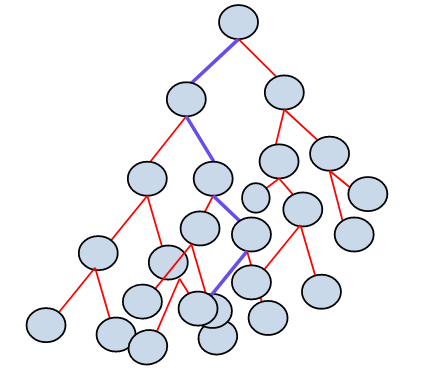
\includegraphics[scale = 0.3]{img/highvar.png}
    \end{columns}
\end{frame}
\begin{frame}{High Variance of gradient estimates}
    \begin{columns}
        \column {0.6\textwidth}
        \begin{itemize}
            \item Using discount factor also reduces the variance to an extent since it diminishes the importance of future rewards.
            \item However these 2 tricks are not always sufficient to solve the problem.
            \item One way of reducing variance which is mostly used in practice is by subtracting the Q value estimate with an appropriate baseline.
            \item Actor critic methods (A2C, A3C) learn a baseline to reduce the variance. (Will be discussed in next tutorial)
        \end{itemize}
        \column{0.4\textwidth}
        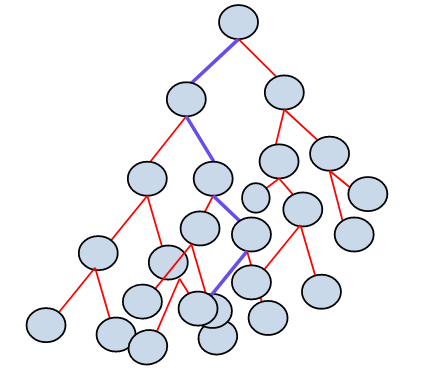
\includegraphics[scale = 0.3]{img/highvar.png}
    \end{columns}    
\end{frame}

\begin{frame}{Sample Efficiency}
    \begin{columns}
        \column{0.5\textwidth}
        \begin{itemize}
            \item The vanilla policy gradient algorithm has a very bad sample efficiency.
            \item The collected trajectories can only be used for a single gradient update.
            \item After making the update we throw away the data that was collected and collect new experience using the updated policy for the next update.
            \item In many cases collecting data might be very expensive (for eg. In Robotics)
        \end{itemize}
        \column{0.5\textwidth}
        
\includegraphics[scale = 0.35]{img/thanos.png}
    \end{columns}
\end{frame}
\begin{frame}{Sample Efficiency}
\begin{itemize}
    \item To better understand why this problem occurs, lets look again at the equation of policy gradients: $\nabla_\theta \mathop{\mathbb{E}_\tau}[R] = \mathop{\mathbb{E}_\tau}[ \nabla_\theta \sum_{t=0}^{T-1}\log\pi(a_t|s_t;\theta)\sum_{t' = t}^{T-1} \gamma^{t'} r_{t'}]$
    \item The expectation is over the trajectory distribution which is a function of policy. 
    \item Once we update the policy, the trajectory distribution will change too.
    \item Hence the collected samples will no longer be valid to compute this expectation.
    \item Variants of vanilla policy gradients like TRPO, PPO (next tutorial) modify the policy gradient to enable multiple policy updates using the collected samples.
    \item Off policy variants like DDPG enables the use of experience replay which helps in using the samples from past experience to make policy updates.
\end{itemize}
\end{frame}